% This is text associated with the open textbook "Open Electromagnetics"
% See immediately below for author, date
% This work is licensed under the Creative Commons Attribution-ShareAlike 4.0 International License. (CC BY-SA 4.0) 
% To view a copy of the license, visit http://creativecommons.org/licenses/by-sa/4.0/

%ORB TITLE Electromagnetic Induction
%ORB AUTHOR 0        # S.W. Ellingson, Virginia Tech (ellingson@vt.edu)
%ORB DATE 20180807   # yyyymmdd
%ORB ABSTRACT Electromagnetic induction and Lenzs' Law

\label{m0129_Electromagnetic_Induction} % <-- Must match name of this file and module directory name.  Don't mess with this!
\index{induction|(}

When an electrically-conducting structure is exposed to a time-varying magnetic field, an electrical potential difference is induced across the structure.
This phenomenon is known as \emph{electromagnetic induction}. 
A convenient introduction to electromagnetic induction is provided by Lenz's Law.
\index{Lenz's law}
This section explains electromagnetic induction in the context of Lenz's Law and provides two examples.

Let us begin with the example depicted in
Figure~\ref{m0129_fLenzLaw}, involving a cylindrical coil.  
Attached to the terminals of the coil is a resistor for which we may identify an electric potential difference $V$ and current $I$.
In this particular case, the sign conventions indicated for $V$ and $I$ are arbitrary, but it is important to be consistent once they are established.
%
\begin{figure}
\begin{center}
\pdftooltip{{  % note double braces
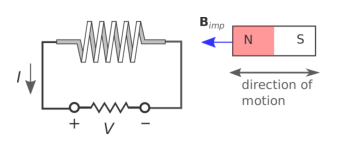
\includegraphics[width=\columnwidth]{modules/m0129_fLenzLaw.eps}
% URL
}}{A circular coil consisting of N turns wound uniformly lies in a rectangular series circuit with a resistor, V, between positive and negative nodes. The current is moving from the coil in a counterclockwise direction. To the right of the coil is a horizontal bar magnet, with the north side pointing toward the coil. A blue vector extends from the magnet toward the coil, labeled B sub imp. Under the magnet is a horizontal double headed arrow, labeled "direction of motion".}
\end{center} 
\centerline{\scriptsize 
\hyperref[m0129_fLenzLaw_credit]{Y.\ Qin} (modified) 
\href{https://creativecommons.org/licenses/by/4.0/}{CC BY 4.0} 
} 
\caption{
\label{m0129_fLenzLaw}
An experiment demonstrating electromagnetic induction and Lenz's Law.
}
\end{figure}

Now let us introduce a bar magnet as shown in Figure~\ref{m0129_fLenzLaw}.
The magnet is centered along the axis of coil, to the right of the coil, and with its north pole facing toward the coil.
The magnet is responsible for the magnetic flux density ${\bf B}_{imp}$.
We refer to ${\bf B}_{imp}$ as an \emph{impressed} magnetic field because this field exists independently of any response that may be induced by interaction with the coil.
Note that ${\bf B}_{imp}$ points to the left inside the coil.

The experiment consists of three tests.
We will find in two of these tests that current flows (i.e., $\left|I\right|>0$), and subsequently, there is an \emph{induced} magnetic field ${\bf B}_{ind}$ due to this current.
It is the direction of the current and subsequently the direction of ${\bf B}_{ind}$ inside the coil that we wish to observe.
The findings are summarized below and in Table~\ref{m0129_tLenzLaw}.
%
\begin{itemize}
\item When the magnet is motionless, we have the unsurprising result that there is no current in the coil. Therefore, no magnetic field is induced, and the total magnetic field is simply equal to ${\bf B}_{imp}$.
\item When the magnet moves \emph{toward} the coil, we observe current that is positive with respect to the reference direction indicated in Figure~\ref{m0129_fLenzLaw}.  This current creates an induced magnetic field ${\bf B}_{ind}$ that points to the \emph{right}, as predicted by magnetostatic considerations from the right-hand rule. Since ${\bf B}_{imp}$ points to the left, it appears that the induced current is opposing the increase in the magnitude of the total magnetic field. 
\item When the magnet moves \emph{away} from the coil, we observe current that is negative with respect to the reference direction indicated in Figure~\ref{m0129_fLenzLaw}.  This current yields ${\bf B}_{ind}$ that points to the \emph{left}. Since ${\bf B}_{imp}$ points to the left, it appears that the induced current is opposing the decrease in the magnitude of the total magnetic field.
\end{itemize}
%
\begin{table*}
\begin{center}
\begin{tabular}{llll}
Magnet is ... & $\left|{\bf B}_{imp}\right|$ in coil is ... & Circuit Response & ${\bf B}_{ind}$ inside coil \\
\hline
Motionless & constant & $V=0$, $I=0$ & none \\
Moving toward coil & increasing & $V>0$, $I>0$ & Pointing right \\
Moving away from coil & decreasing & $V<0$, $I<0$ & Pointing left \\
\end{tabular}
\end{center}
\caption{\label{m0129_tLenzLaw}Results of the experiment associated with Figure~\ref{m0129_fLenzLaw}.}
\end{table*}

The first conclusion one may draw from this experiment is that changes in the magnetic field can induce current.  
This was the claim made in the first paragraph of this section and is a consequence of Faraday's Law, 
\index{Faraday's law}
which is tackled in detail in Section~\ref{m0055_Faradays_Law}.
The second conclusion -- also associated with Faraday's Law -- is the point of this section:  The induced magnetic field -- that is, the one due to the current induced in the coil -- always opposes the change in the impressed magnetic field.  Generalizing:
%
%ORB HIGHLIGHT
\begin{mdframed}[backgroundcolor=yellow!20] 
Lenz's Law states that the current that is induced by a change in an impressed magnetic field creates an induced magnetic field that opposes (acts to reduce the effect of) the change in the total magnetic field.
\end{mdframed}

When the magnet moves, three things happen: (1) A current is induced, (2) A magnetic field is induced (which adds to the impressed magnetic field), and (3) the value of $V$ becomes non-zero.
Lenz's Law does not address which of these are responding directly to the change in the impressed magnetic field, and which of these are simply responding to changes in the other quantities.
Lenz's Law may leave you with the incorrect impression that it is $I$ that is induced, and that ${\bf B}_{ind}$ and $V$ are simply responding to this current.
In truth, the quantity that is induced is actually $V$.  
This can be verified in the above experiment by replacing the resistor with a high-impedance voltmeter, which will indicate that $V$ is changing even though there is negligible current flow.
Current flow is simply a response to the induced potential.
Nevertheless, it is common to say informally that ``$I$ is induced,'' even if it is only indirectly through $V$. 

So, if Lenz's Law is simply an observation and not an explanation of the underlying physics, then what is it good for?
Lenz's Law is often useful for quickly determining the direction of current flow in practical electromagnetic induction problems, without resorting to the mathematics associated with Faraday's Law.
Here's an example:

%%%%%%%%%%%%%%%%%%%%%%%%%%%%%%%%%%%%%%%%%%%%%%%
%ORB EXAMPLE
~\\ \begin{example} 
\begin{mdframed}[backgroundcolor=brown!20,linecolor=brown!20]\raggedright
Electromagnetic induction through a transformer.
\index{transformer!induction}
\\~\\
Figure~\ref{m0129_fLLCoil} shows a rudimentary circuit consisting of a battery and a switch on the left, a voltmeter on the right, and a transformer linking the two.
It is not necessary to be familiar with transformers to follow this example; suffice it to say, the transformer considered here consists of two coils wound around a common toroidal core, which serves to contain magnetic flux.  In this way, the flux generated by either coil is delivered to the other coil with negligible loss.

The experiment begins with the switch on the left in the open state.  
Thus, there is no current and no magnetic field apparent in the coil on the left.
The voltmeter reads 0~V.
When the switch is closed, what happens?

{\bf Solution.}  Closing the switch creates a current in the coil on the left. 
Given the indicated polarity of the battery, this current flows counter-clockwise through the circuit on the left, with current arriving in the left coil through the bottom terminal. 
Given the indicated direction of the winding in the left coil, the impressed magnetic field ${\bf B}_{imp}$ is oriented counter-clockwise through the toroidal core. 
The coil on the right ``sees'' ${\bf B}_{imp}$ increase from zero to some larger value.
Since the voltmeter presumably has input high impedance, negligible current flows.
However, if current were able to flow, Lenz's Law dictates that it would be induced to flow in a counter-clockwise direction around the circuit on the right, since the induced magnetic field ${\bf B}_{ind}$ would then be clockwise-directed so as to oppose the increase in ${\bf B}_{imp}$.
Therefore, the potential measured at the bottom of the right coil would be higher than the potential at the top of the right coil. 
The figure indicates that the voltmeter measures the potential at its right terminal relative to its left terminal, so the needle will deflect to the right.
This deflection will be temporary, since the current provided by the battery becomes constant at a new non-zero value and ${\bf B}_{ind}$ responds only to the \emph{change} in ${\bf B}_{imp}$.  
The voltmeter reading will remain at zero for as long as the switch remains closed and the current remains steady.

%%% TODO: Make these problems
Here are some follow up exercises to test your understanding of what is going on:
(1) Now open the switch.  What happens?
(2) Repeat the original experiment, but before starting, swap the terminals on the battery.  
\end{mdframed}
%
\begin{figure}
\begin{center}
\pdftooltip{{  % note double braces
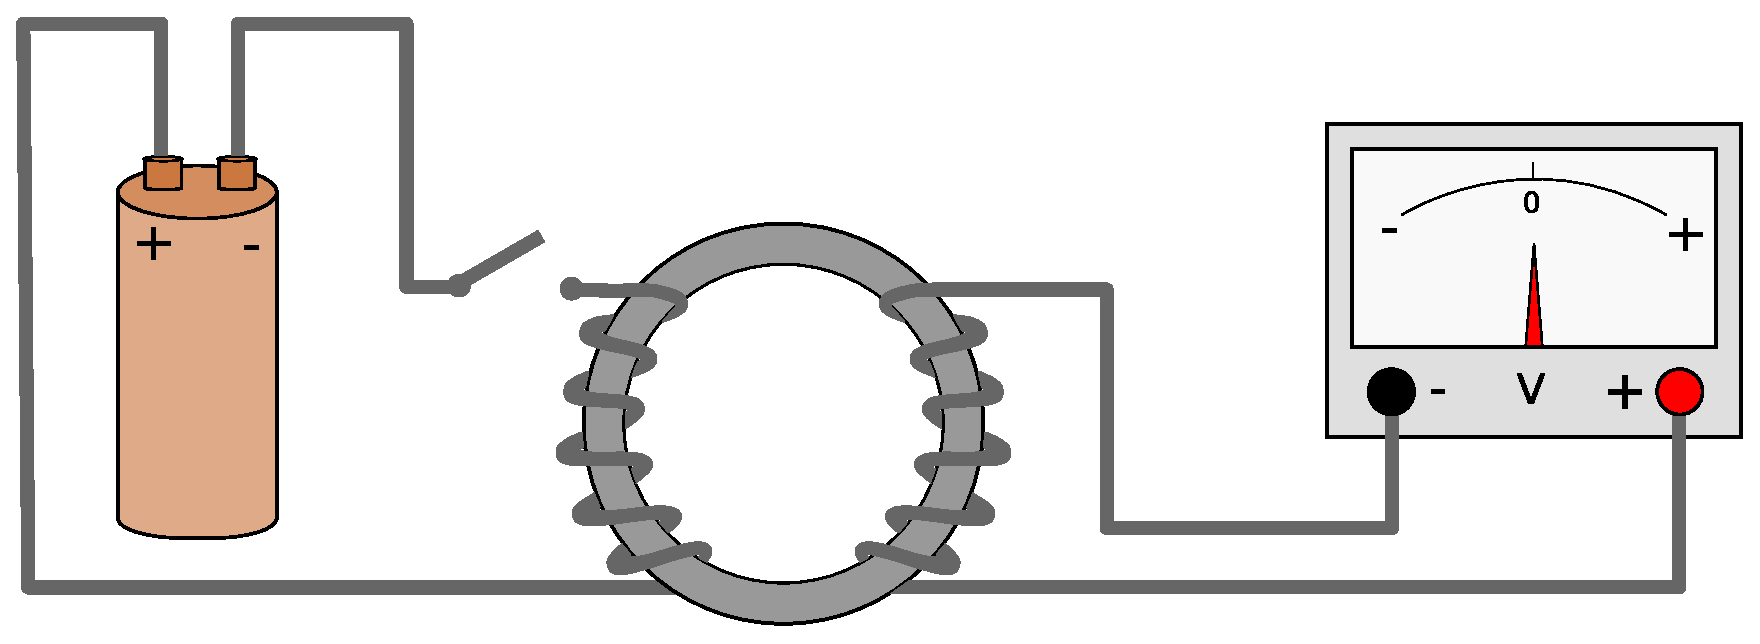
\includegraphics[width=\columnwidth]{modules/m0129_fLLCoil.eps}
% https://commons.wikimedia.org/wiki/File:Faraday_emf_experiment.svg
}}{Wire comes from the negative side of the battery and winds around one side of the loop and returns to the positive side of the battery. Wire runs around the opposite side of the loop and connects to the positive and negative leads of a voltmeter.}
\end{center} 
\centerline{\scriptsize 
\hyperref[m0129_fLLCoil_Credit]{E.\ Bach} 
\href{https://creativecommons.org/publicdomain/zero/1.0/deed.en}{CC0 1.0} (modified) 
} 
\caption{
Electromagnetic induction through a transformer.
}
\label{m0129_fLLCoil}
\end{figure}
\end{example}
%%%%%%%%%%%%%%%%%%%%%%%%%%%%%%%%%%%%%%%%%%%%%%%

Finally, it is worth noting that Lenz's law can also be deduced from the principle of conservation of energy.
The argument is that if the induced magnetic field \emph{reinforced} the change in the impressed magnetic field, then the sum magnetic field would increase.  This would result in a further increase in the induced magnetic field, leading to a positive feedback situation.  However, positive feedback cannot be supported without an external source of energy, leading to a logical contradiction.  In other words, the principle of conservation of energy requires the \emph{negative} feedback described by Lenz's law.      

{\bf Additional Reading:}
\begin{itemize}
\item ``\href{https://en.wikipedia.org/wiki/Electromagnetic_induction}{Electromagnetic Induction}'' on Wikipedia.
\item ``\href{https://en.wikipedia.org/wiki/Lenz's_law}{Lenz's Law}'' on Wikipedia.
\end{itemize}

\index{induction|)}


